\chapter*{Introduction}
\addstarredchapter{Introduction}
\renewcommand\chapterillustration{INT/INT}
\ThisULCornerWallPaper{1}{\chapterillustration}

\lettrine[lines=4, slope=-0.5em,nindent=10pt]{L}{e} détecteur \textit{Compact Muon Solenoid} (CMS) est un détecteur généraliste placé sur la ligne du faisceau du collisionneur \textit{Large Hadron Collider} situé à l'Organisation Européenne pour la Recherche Nucléaire (CERN). Il a permit de produire d'excellent résultats scientifique\footnote{Plus de \num{600} papiers ont été publiés} et notamment la découverte du boson de Higgs en \num{2012} (cd.fig~\ref{higgs}) conjointement avec le détecteur \textit{A Toroidal LHC ApparatuS} (ATLAS). 


\begin{figure}[ht!]
	\centering
	\subfloat[Distribution de la masse invariante en diphoton. Chaque événement est affecté du poids $S/(S+B)$. de sa catégorie. Les lignes représentent l'ajustement du bruit de fond et du signal et les bandes colorées représentent les déviations standard du bruit de fond à $\pm1$ et $\pm 2 \sigma$.]{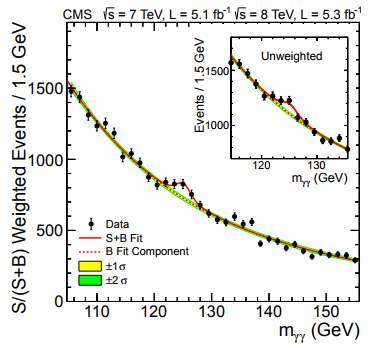
\includegraphics[width=0.49\textwidth]{INT/higgs1.png}}
	\hfill
	\subfloat[Distribution de la masse invariante pour l'analyse $ZZ->4l$. Les points représentent les données, les histogrammes pleins le bruit de fond et l'histogramme creu montre le signal attendu pour un boson de Higgs de masse $M_{H}=\SI{125}{\giga\eV}$ ajouté au bruit de fond attendu. ]{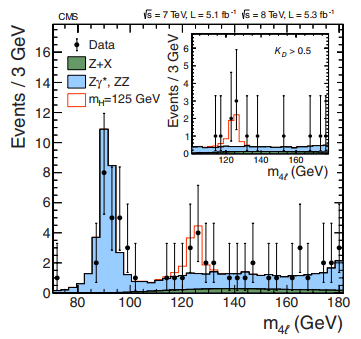
\includegraphics[width=0.49\textwidth]{INT/higgs2.png}}
	\caption{Les deux canaux de désintégration du boson de Higgs ayant permis sa découverte dans l'expérience CMS.}
	\label{higgs}
\end{figure}

Cependant, aucune trace de nouvelle physique n'a été trouvée. Afin d'améliorer la capacité de détection d'une nouvelle physique, le LHC va subir une mise à niveau en \num{2026} afin d'augmenter sa luminosité instantanée par un facteur \num{5} à \num{7.5} et sera renommé pour l'occasion \textit{High Luminosity Large Hadron Collider} (HL-LHC). L'augmentation de la luminosité du LHC aura des conséquences importantes pour les détecteurs placés sur sa ligne de faisceaux (augmentation de l'empilement et du flux de particules produites lors des collisions etc.). Afin de faire face à l'augmentation du taux de collision et de profiter de cette augmentation de luminosité instantanée, le détecteur CMS doit être mis à niveau. 

Cette thèse se concentre sur la mise à niveau du trajectographe à muons de CMS est plus particulièrement sur l'instrumentation de zones de ce trajectographe par des Resistive Plate Chamber (RPC) de nouvelle génération capable de supporter les flux de particules parcourant ces zones. 



